\documentclass[aspectratio=169,10pt]{beamer}

\usepackage[utf8]{inputenc}
\usepackage[T1]{fontenc}
\usepackage{lmodern}
\usepackage{amsmath,amssymb}
\usepackage{booktabs}
\usepackage{array}
\usepackage{tikz}
\usepackage{graphicx}
\usetikzlibrary{arrows.meta,positioning,shapes.geometric,fit,calc}
\usepackage{ragged2e}

% Paleta alinhada ao pipeline InovAI / PepMem
\definecolor{InovGreen}{RGB}{68,40,155}
\definecolor{InovLightGreen}{RGB}{242,239,253}
\definecolor{InovDark}{RGB}{40,36,55}
\definecolor{InovGray}{RGB}{248,247,252}
\definecolor{InovOrange}{RGB}{122,113,245}
\definecolor{InovBlue}{RGB}{92,116,255}
\definecolor{PmGreen}{RGB}{47,125,74}
\definecolor{PmMembrane}{RGB}{30,92,90}

\setbeamertemplate{navigation symbols}{}
\setbeamertemplate{itemize item}{\color{InovGreen}$\blacktriangleright$}
\setbeamertemplate{itemize subitem}{\color{InovOrange}$\bullet$}
\setbeamertemplate{enumerate item}{\color{InovGreen}\insertenumlabel.}
\setbeamercolor{title}{fg=InovGreen}
\setbeamercolor{frametitle}{fg=InovGreen,bg=white}
\setbeamercolor{block title}{fg=white,bg=InovGreen}
\setbeamercolor{block body}{fg=InovDark,bg=InovLightGreen}
\setbeamercolor{alerted text}{fg=InovOrange}

\setbeamertemplate{frametitle}{%
  \vspace{-0.05cm}
  \insertframetitle
  \par\vspace{-0.1cm}
  {\color{InovGreen}\rule{\linewidth}{0.5pt}}
}

\setbeamertemplate{footline}{%
  \hfill{\color{InovDark}\scriptsize
  PepMem-AI \;·\; \insertframenumber/\inserttotalframenumber\hspace{0.4cm}}
  \vspace{0.15cm}
}

\tikzset{
  box/.style={rectangle, rounded corners=3pt, draw=InovGreen, very thick,
    align=center, fill=InovLightGreen, minimum height=0.7cm, text width=2.4cm, font=\scriptsize},
  orangebox/.style={rectangle, rounded corners=3pt, draw=InovOrange, very thick,
    align=center, fill=orange!10, minimum height=0.7cm, text width=2.4cm, font=\scriptsize},
  bluebox/.style={rectangle, rounded corners=3pt, draw=InovBlue, very thick,
    align=center, fill=blue!8, minimum height=0.7cm, text width=2.4cm, font=\scriptsize},
  grebox/.style={rectangle, rounded corners=3pt, draw=PmGreen, very thick,
    align=center, fill=green!8, minimum height=0.7cm, text width=2.4cm, font=\scriptsize},
  arrow/.style={-{Latex[length=2.2mm]}, very thick, draw=InovDark}
}

\title[Modelagem PepMem-AI]{PepMem-AI: dados, modelagem e resultados}
\subtitle{Predição de alta atividade antimicrobiana (peptídeo $\times$ membrana)}
\author{InovAI Lab \;·\; UFRN}
\institute{PoC computacional --- baseline RF + multimodal RF/ESM-2}
\date{2026}

\begin{document}

% ----------------------------------------------------------------
\begin{frame}[plain]
  \vspace{1.2cm}
  {\color{InovGreen}\Large\bfseries PepMem-AI}\\[0.35cm]
  {\large Dados, modelagem e resultados}\\[0.6cm]
  {\color{InovDark}
  Priorização in silico de peptídeos escorpiônicos\\
  antes da validação experimental in vitro}\\[1.0cm]
  {\small InovAI Lab / LANCE --- IMD/UFRN}\\[0.2cm]
  {\scriptsize Métricas dos artefatos em \texttt{data/processed/models/} (treino commitado)}
\end{frame}

% ----------------------------------------------------------------
\begin{frame}{Agenda}
\begin{enumerate}
  \item Problema e pergunta do modelo
  \item Dados: fontes, volume e rótulo
  \item Features: clássicas, PMI e ESM-2
  \item Modelagem: RF, LOPO e calibração
  \item Resultados (baseline e multimodal)
  \item Uso: dashboard, API e deploy
  \item Limitações e próximos passos
\end{enumerate}
\end{frame}

% ----------------------------------------------------------------
\begin{frame}{Problema}
\begin{block}{Contexto}
Peptídeos de \emph{Tityus stigmurus} (Stigmurin e análogos) interagem com membranas
diversas (Gram+/Gram$-$, fungo, célula mamífera). Testar todos os pares in vitro é caro.
\end{block}
\vspace{0.3cm}
\begin{columns}[T]
\begin{column}{0.55\textwidth}
\textbf{Pergunta operacional}\\[0.2cm]
\begin{itemize}
  \item Dado peptídeo + membrana-alvo,
  \item qual a chance de \alert{alta atividade}?
  \item Rótulo: MIC $\le$ \textbf{3,4\,µM}
\end{itemize}
\end{column}
\begin{column}{0.42\textwidth}
\begin{block}{Papel do PoC}
Priorizar candidatos.\\
Não substitui MIC,\\
hemólise nem clínica.
\end{block}
\end{column}
\end{columns}
\end{frame}

% ----------------------------------------------------------------
\begin{frame}{De onde veio o desenho}
\begin{columns}[T]
\begin{column}{0.52\textwidth}
\begin{block}{Pipeline InovAI (Nível 1)}
Baselines: RF, XGBoost, SVM, logreg.\\[0.15cm]
Com poucos dados: classificador +\\
encoder congelado; PMI + SHAP.
\end{block}
\vspace{0.25cm}
\begin{block}{PoC implementado}
\textbf{RF} (baseline e multimodal).\\
ESM-2 \texttt{t6\_8M} como embedding.\\
SHAP TreeExplainer no dashboard.
\end{block}
\end{column}
\begin{column}{0.45\textwidth}
\begin{block}{Proposta CNPq (horizonte)}
Deep learning multimodal\\
(MLP / Transformers).\\[0.15cm]
{\scriptsize Meta de médio/longo prazo;\\
não é o modelo em produção no Cloud.}
\end{block}
\end{column}
\end{columns}
\end{frame}

% ----------------------------------------------------------------
\begin{frame}{Dados --- fontes}
\begin{center}
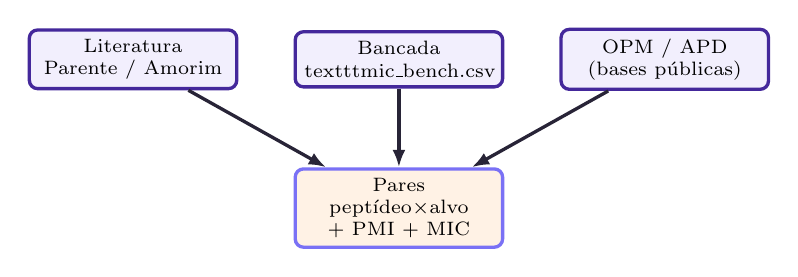
\begin{tikzpicture}[
  node distance=0.55cm and 0.7cm,
  every node/.style={font=\scriptsize}
]
  \node[box] (lit) {Literatura\\Parente / Amorim};
  \node[box, right=of lit] (bench) {Bancada\\texttt{mic\_bench.csv}};
  \node[box, right=of bench] (opm) {OPM / APD\\(bases públicas)};
  \node[orangebox, below=1.0cm of bench] (pairs) {Pares peptídeo$\times$alvo\\+ PMI + MIC};
  \draw[arrow] (lit) -- (pairs);
  \draw[arrow] (bench) -- (pairs);
  \draw[arrow] (opm) -- (pairs);
\end{tikzpicture}
\end{center}
\vspace{0.35cm}
\begin{itemize}
  \item Bancada \textbf{sobrescreve} literatura no mesmo par (\texttt{import\_bench\_mic.py}).
  \item Distribuição atual dos MICs: \textbf{78} bancada + \textbf{12} literature $=$\textbf{90}.
  \item Alvos com MIC: \textbf{18} membranas distintas.
\end{itemize}
\end{frame}

% ----------------------------------------------------------------
\begin{frame}{Dados --- volume e rótulo}
\begin{columns}[T]
\begin{column}{0.48\textwidth}
\begin{block}{Conjunto de treino}
\begin{itemize}
  \item \textbf{90} pares com MIC
  \item \textbf{10} peptídeos distintos
  \item Taxa positiva: \textbf{44,4\%}
\end{itemize}
\end{block}
\end{column}
\begin{column}{0.48\textwidth}
\begin{block}{Rótulo binário}
\[
y = \begin{cases}
1 & \text{se MIC} \le 3{,}4\,\mu\text{M}\\
0 & \text{caso contrário}
\end{cases}
\]
{\scriptsize Limiar operacional do projeto\\
(valores ativos em Parente 2022).}
\end{block}
\end{column}
\end{columns}
\vspace{0.4cm}
\begin{center}
{\small Mediana dos MICs $\approx$ 4,7\,µM --- o corte 3,4\,µM \emph{não} é a mediana.}
\end{center}
\end{frame}

% ----------------------------------------------------------------
\begin{frame}{Features --- baseline (11)}
\begin{columns}[T]
\begin{column}{0.55\textwidth}
\begin{itemize}
  \item Peptídeo: $q$, $h$, $\mu H$
  \item Membrana: carga superficial, fração aniônica, colesterol, LPS, peptidoglicano, ergosterol, envelope viral
  \item \textbf{PMI} (índice interpretável)
\end{itemize}
\vspace{0.25cm}
{\scriptsize
\[
\text{PMI} = \alpha\,q_p|q_m| + \beta\,h_p h_m + \gamma\,\mu H_p - \delta\,\text{col}_m
\]
$\alpha{=}1{,}0$, $\beta{=}0{,}5$, $\gamma{=}0{,}3$, $\delta{=}0{,}4$}
\end{column}
\begin{column}{0.42\textwidth}
\begin{block}{Carga se não informada}
Soma simplificada a pH\,$\sim$7:\\
K,R $= +1$; H $= +0{,}1$;\\
D,E $= -1$.
\end{block}
\end{column}
\end{columns}
\end{frame}

% ----------------------------------------------------------------
\begin{frame}{Features --- multimodal (+ ESM-2)}
\begin{itemize}
  \item Embedding: \texttt{facebook/esm2\_t6\_8M\_UR50D}
  \item Agregação: \textbf{mean-pooling} dos resíduos $\rightarrow$ vetor $\sim$\textbf{320} dims
  \item Entrada do RF: 11 clássicas + 320 $\approx$ \textbf{331} features
  \item Artefato: \texttt{data/processed/embeddings/esm2\_all.npz}
\end{itemize}
\vspace{0.35cm}
\begin{block}{Por que t6 8M?}
Feito para proteínas; só precisa da sequência; cabe em CPU / HF Space;\\
complementa o PMI sem exigir estrutura 3D.
\end{block}
\end{frame}

% ----------------------------------------------------------------
\begin{frame}{Pipeline de modelagem}
\begin{center}
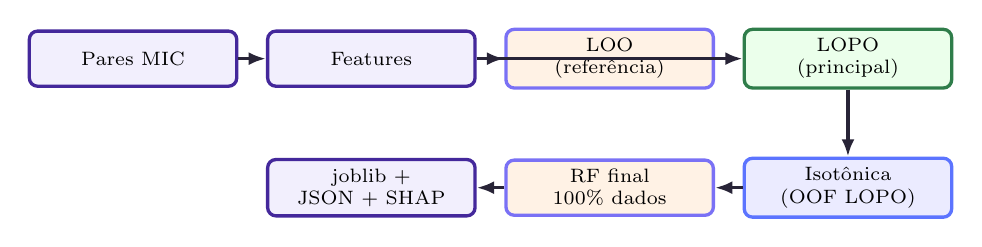
\begin{tikzpicture}[node distance=0.45cm and 0.35cm, every node/.style={font=\scriptsize\bfseries}]
  \node[box] (d) {Pares MIC};
  \node[box, right=of d] (f) {Features};
  \node[orangebox, right=of f] (loo) {LOO\\(referência)};
  \node[grebox, right=of loo] (lopo) {LOPO\\(principal)};
  \node[bluebox, below=0.85cm of lopo] (cal) {Isotônica\\(OOF LOPO)};
  \node[orangebox, left=of cal] (rf) {RF final\\100\% dados};
  \node[box, left=of rf] (art) {joblib +\\JSON + SHAP};
  \draw[arrow] (d) -- (f);
  \draw[arrow] (f) -- (loo);
  \draw[arrow] (f) -- (lopo);
  \draw[arrow] (lopo) -- (cal);
  \draw[arrow] (cal) -- (rf);
  \draw[arrow] (rf) -- (art);
\end{tikzpicture}
\end{center}
\vspace{0.45cm}
\begin{itemize}
  \item Pipeline: \texttt{StandardScaler} $\rightarrow$ \texttt{RandomForestClassifier}
  \item Baseline: 200 árvores; multimodal: 300 árvores, \texttt{max\_depth}=6
  \item \texttt{class\_weight='balanced'}
\end{itemize}
\end{frame}

% ----------------------------------------------------------------
\begin{frame}{Validação: LOO vs LOPO}
\begin{columns}[T]
\begin{column}{0.48\textwidth}
\begin{block}{LOO (por amostra)}
Tira \textbf{1 par} por vez.\\[0.15cm]
O mesmo peptídeo pode\\
ficar no treino (outro alvo).\\[0.15cm]
{\scriptsize AUC mais otimista\\
(vazamento por homologia).}
\end{block}
\end{column}
\begin{column}{0.48\textwidth}
\begin{block}{LOPO (por peptídeo)}
Tira \textbf{todo} o peptídeo.\\[0.15cm]
Generalização para sequência\\
nunca vista.\\[0.15cm]
{\scriptsize Métrica principal +\\
probs OOF para calibração.}
\end{block}
\end{column}
\end{columns}
\vspace{0.35cm}
\begin{center}
{\small Família Stigmurin: análogos $\sim$94\% idênticos $\Rightarrow$ LOPO é essencial.}
\end{center}
\end{frame}

% ----------------------------------------------------------------
\begin{frame}{Calibração isotônica}
\begin{itemize}
  \item RF ordena bem, mas \texttt{predict\_proba} é \textbf{voto do ensemble}, não frequência real.
  \item Com $\sim$90 MICs, probs brutas tendem a polarizar (0/1).
  \item \textbf{IsotonicRegression} nas probs OOF do LOPO $\rightarrow$ $p_{\text{calibrada}}$.
  \item Preserva a ordem dos candidatos; alinha \% do dashboard ao LOPO.
\end{itemize}
\vspace{0.3cm}
\begin{block}{Inferência}
$p_{\text{bruta}} = \mathrm{RF.predict\_proba}$\quad$\rightarrow$\quad
$p_{\text{calibrada}} = \mathrm{calibrator.predict}([p_{\text{bruta}}])$
\end{block}
\end{frame}

% ----------------------------------------------------------------
\begin{frame}{Resultados --- Baseline RF}
\begin{center}
\renewcommand{\arraystretch}{1.25}
\begin{tabular}{lcc}
\toprule
\textbf{Métrica} & \textbf{LOO} & \textbf{LOPO} \\
\midrule
AUC & 0,878 & \textbf{0,878} \\
Acurácia & 0,833 & 0,744 \\
F1 (classe positiva) & 0,828 & 0,729 \\
\bottomrule
\end{tabular}
\end{center}
\vspace{0.45cm}
\begin{itemize}
  \item Modelo: 11 features clássicas + PMI
  \item Deploy: Streamlit Cloud (sem PyTorch)
  \item Calibração: isotônica sobre OOF LOPO
\end{itemize}
\end{frame}

% ----------------------------------------------------------------
\begin{frame}{Resultados --- Multimodal RF + ESM-2}
\begin{center}
\renewcommand{\arraystretch}{1.25}
\begin{tabular}{lcc}
\toprule
\textbf{Métrica} & \textbf{LOO} & \textbf{LOPO} \\
\midrule
AUC & 0,845 & \textbf{0,809} \\
\bottomrule
\end{tabular}
\end{center}
\vspace{0.4cm}
\begin{itemize}
  \item 331 features (clássicas + embedding)
  \item LOPO cai mais que o baseline: embedding captura similaridade de sequência;\\
        sem o peptídeo no treino, generaliza um pouco pior nesta família pequena
  \item Deploy: Hugging Face Space / local com \texttt{requirements-space.txt}
\end{itemize}
\end{frame}

% ----------------------------------------------------------------
\begin{frame}{AUC LOPO por peptídeo (baseline)}
\begin{center}
\renewcommand{\arraystretch}{1.15}
{\scriptsize
\begin{tabular}{lc|lc}
\toprule
\textbf{ID} & \textbf{AUC} & \textbf{ID} & \textbf{AUC} \\
\midrule
P11 & 0,90 & P15 & 0,83 \\
P12 & 0,95 & P16 & 0,95 \\
P13 & 0,88 & P17 & 0,80 \\
P14 & 0,88 & P18 & 0,67 \\
\bottomrule
\end{tabular}}
\end{center}
\vspace{0.35cm}
\begin{itemize}
  \item P05 e P10: AUC por peptídeo indefinida (uma só classe no fold)
  \item Variabilidade entre análogos --- amostra ainda limitada
\end{itemize}
\end{frame}

% ----------------------------------------------------------------
\begin{frame}{Explicabilidade e produto}
\begin{columns}[T]
\begin{column}{0.48\textwidth}
\begin{block}{SHAP}
TreeExplainer no RF.\\
Beeswarm global + local.\\
Dims ESM agregadas no gráfico.
\end{block}
\vspace{0.2cm}
\begin{block}{Dashboard}
Predição única / lote FASTA\\
Ranking multi-alvo\\
Relatórios MD/DOCX/PDF
\end{block}
\end{column}
\begin{column}{0.48\textwidth}
\begin{block}{Onde roda}
Cloud: baseline leve\\
Space HF: multimodal\\
API FastAPI (opcional)
\end{block}
\vspace{0.2cm}
\begin{block}{Docs}
\texttt{docs/TREINO.md}\\
\texttt{docs/INTERPRETACAO\_RESULTADOS.md}
\end{block}
\end{column}
\end{columns}
\end{frame}

% ----------------------------------------------------------------
\begin{frame}{Limitações}
\begin{itemize}
  \item Poucos peptídeos distintos ($\sim$10 com MIC) --- LOPO ajuda, mas amostra é pequena
  \item Limiar 3,4\,µM é escolha de projeto, não padrão CLSI
  \item Hemólise existe nos pares, mas o RF classifica \textbf{atividade MIC}, não toxicidade direta
  \item Multimodal ainda é RF+ESM, não o encoder multimodal completo da proposta CNPq
  \item Predição \textbf{prioriza} ensaio; não substitui bancada
\end{itemize}
\end{frame}

% ----------------------------------------------------------------
\begin{frame}{Mensagens-chave}
\begin{enumerate}
  \item \textbf{Dados:} 90 MICs (bancada + literatura), rótulo MIC $\le$ 3,4\,µM
  \item \textbf{Modelo:} Random Forest (Nível 1 do pipeline InovAI) + PMI; ESM-2 no multimodal
  \item \textbf{Validação:} LOPO é a métrica honesta; isotônica calibra o dashboard
  \item \textbf{Resultado:} baseline LOPO AUC $\approx$ \textbf{0,88}; multimodal LOPO AUC $\approx$ \textbf{0,81}
  \item \textbf{Uso:} priorizar candidatos Stigmurin/análogos antes do in vitro
\end{enumerate}
\end{frame}

% ----------------------------------------------------------------
\begin{frame}[plain]
\vspace{2.2cm}
\begin{center}
{\color{InovGreen}\Large\bfseries Obrigado}\\[0.5cm]
{\large Perguntas}\\[1.0cm]
{\small Código: \texttt{github.com/gbmotta/PepMem-AI}}\\[0.15cm]
{\scriptsize Artefatos: \texttt{baseline\_mic\_loo.json} · \texttt{multimodal\_mic\_loo.json}}
\end{center}
\end{frame}

\end{document}
